\section{Evaluation}
\label{sec:exp}

\subsection{Setup}
The simulator runs a 24-hour horizon with 10 random seeds. Unless otherwise stated, traces use a 90-minute orbit, a 10-minute contact window, and a 35 Mbps downlink. Each trace contains 260 heterogeneous tasks with model scales in $\{1.7,3,8\}$B, log-normal data sizes, urgent and routine half-lives, and configured prefill/decode token counts. The on-board compute-energy budget is 150 kJ and the memory ceiling is 16 GB. The default PRE module uses 18\% of full on-board inference energy/latency, retains 32\% of raw bits, and keeps 94\% of task utility; \Cref{fig:pre} sweeps these assumptions. All numbers and plots are regenerated from CSV files produced on the remote RTX 4090 server.

\subsection{Main Results}
\Cref{fig:value} and \Cref{tab:main} compare Heuristic-TVD with three baselines and the MILP upper bound. All-Downlink loses value because urgent tasks wait for contacts. All-On-Board has low latency but exhausts energy and drops tasks. Fixed-Threshold uses task value but cannot jointly adapt to residual energy, bandwidth, and model memory. Heuristic-TVD reaches $0.90\pm0.01$ normalized value, above All-Downlink ($0.59\pm0.01$), All-On-Board ($0.75\pm0.01$), and Fixed-Threshold ($0.85\pm0.01$), while reporting zero OOM and zero energy violations.

\begin{figure}[tb]
  \centering
  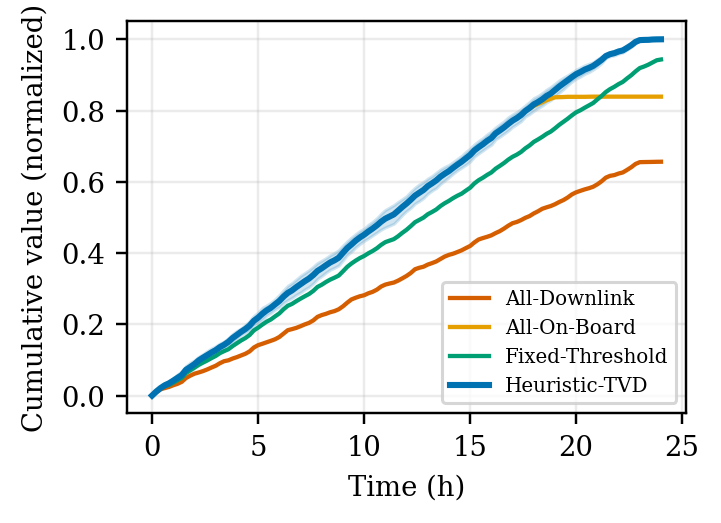
\includegraphics[width=\columnwidth]{figures/value_curve.png}
  \caption{Cumulative realized value over 24 hours. Heuristic-TVD preserves energy for later high-value tasks while still serving urgent tasks early.}
  \label{fig:value}
\end{figure}

\begin{table}[tb]
\centering
\caption{Main 24-hour results over 10 seeds. Value is normalized by the MILP bound; bandwidth saving is relative to All-Downlink.}
\label{tab:main}
\scriptsize
\begin{tabular}{lcccc}
\toprule
Method & Value$\uparrow$ & J/task$\downarrow$ & BW save$\uparrow$ & Lat. med.$\downarrow$\\
\midrule
\MainResultRows
\bottomrule
\end{tabular}
\end{table}

\begin{table}[tb]
\centering
\caption{Action mix in the main experiment. PRE is selected only when partial semantic transfer is more valuable than raw downlink under residual resources.}
\label{tab:mix}
\scriptsize
\begin{tabular}{lcccc}
\toprule
Method & ON & PRE & DOWN & DROP\\
\midrule
\ActionMixRows
\bottomrule
\end{tabular}
\end{table}

\subsection{NTN Contact Sensitivity}
\Cref{fig:network} varies the network regime. At low downlink rates, Heuristic-TVD preserves value by avoiding raw transfers and using ON/PRE for urgent tasks. As contact windows expand, the action mix shifts smoothly because the value-density denominator accounts for both residual energy and bandwidth. This is the key MobiArch point: the policy is an architecture-level adaptation layer, not a single fixed offloading threshold.

\begin{figure}[tb]
  \centering
  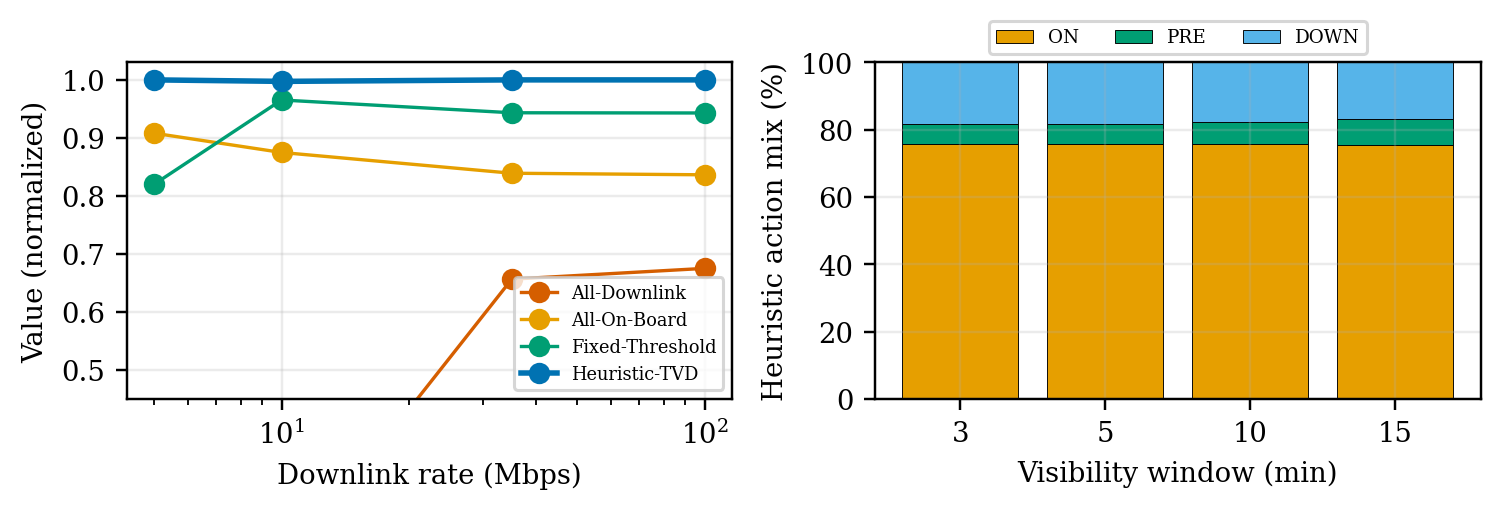
\includegraphics[width=\columnwidth]{figures/network_sensitivity.png}
  \caption{Network/contact sensitivity. Left: value across downlink rates. Right: Heuristic-TVD action mix as visibility windows change.}
  \label{fig:network}
\end{figure}

\subsection{PRE and Hardware Sensitivity}
\Cref{fig:pre} sweeps PRE retained-bit ratio $\rho$ and utility-retention model $\eta(\rho)$. PRE is most useful in the middle regime: aggressive filtering saves bandwidth but can lose value, while large $\rho$ approaches raw downlink. This turns PRE from a black-box assumption into an explicit design space.

\begin{figure}[tb]
  \centering
  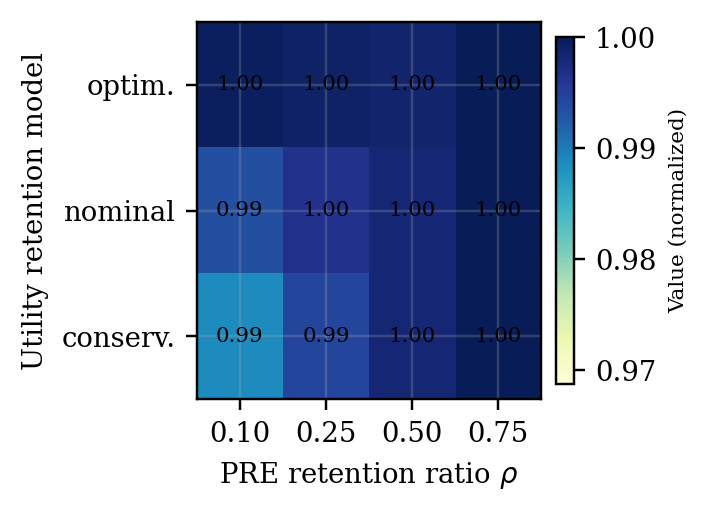
\includegraphics[width=\columnwidth]{figures/pre_sensitivity.png}
  \caption{PRE sensitivity over retained bits and utility-retention regimes. Values are normalized against the best PRE/no-PRE choice for the same seed and setting.}
  \label{fig:pre}
\end{figure}

\Cref{fig:hardware} scales the measured 4090 energy and latency profile by $0.5$--$4\times$. Faster profiles choose full on-board inference; constrained profiles shift toward PRE and DOWN while preserving feasibility. Thus the framework does not rely on the 4090 as target hardware: it consumes a replaceable cost surface.

\begin{figure}[tb]
  \centering
  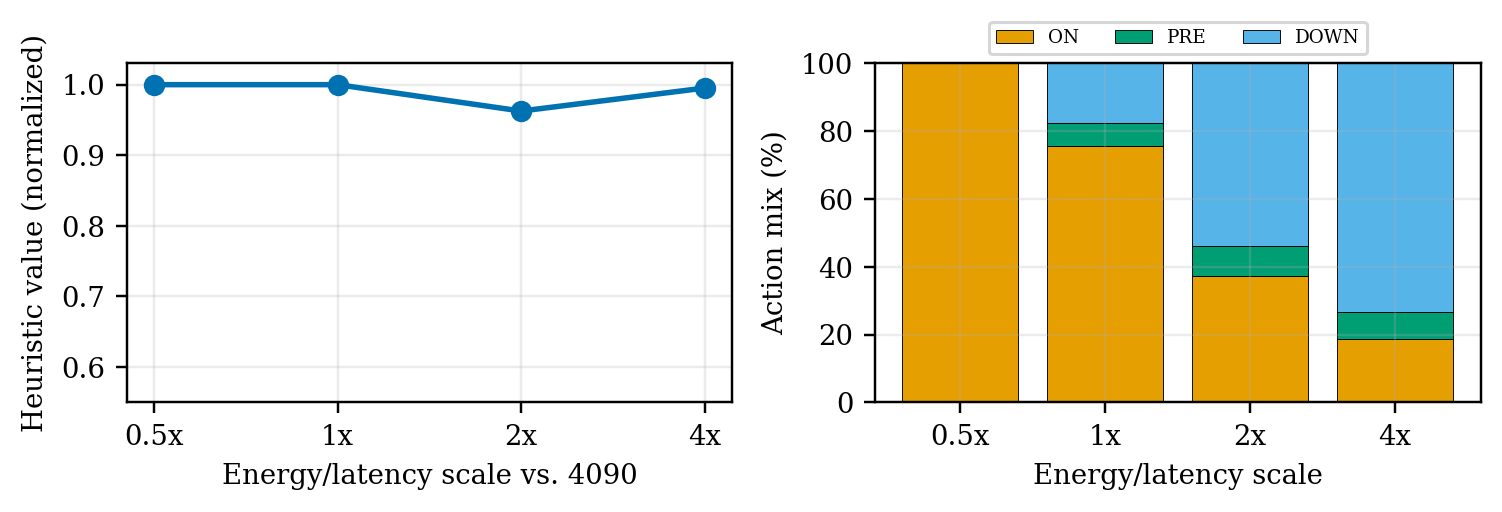
\includegraphics[width=\columnwidth]{figures/hardware_sensitivity.png}
  \caption{Hardware-profile scaling. Heuristic-TVD changes its action mix as the measured profile is scaled from faster accelerators to constrained edge devices.}
  \label{fig:hardware}
\end{figure}
